%!TEX root = /Users/louis/Documents/PhD/Progress Report/pr.tex
\subsection{Study of Existing Data}
In my qualifying dissertation, I identified the need for a categorisation of the evolution of MDE artefacts. A study of example data (existing MDE projects containing evolution) was proposed to produce this categorisation. Work commenced by locating appropriate projects for the study. Several were discarded as they contained too few changes, or an inadequate description of the changes made. Further requirements, discussed below, were devised to determine the suitability of candidate projects. The requirements on candidate projects varied for each type of evolution:

\paragraph{Model and metamodel co-evolution}
A candidate project for the study of model and metamodel co-evolution had to define a metamodel and some adaptation of that metamodel (requirement REQ1). In the projects considered, the metamodel adaptation took the form of either (1) another version of the metamodel, or (2) a change history (which recorded each of the steps used to produce the adapted metamodel).

A candidate project also had to provide example instances of models before and after each migration activity (REQ2).

Ideally, a candidate project included more than one consecutive metamodel adaptation, so as to represent the way in which the same development artefacts can continue to evolve over time (optional requirement OPT1).

\paragraph{Model synchronisation}
A candidate project for the study of model synchronisation had to define a model-to-model transformation (REQ3).

Furthermore, a candidate project had to include many examples of source and target model for that transformation (REQ4).

Crucially, a candidate project had to provide many examples of the kinds of change (to either source or target model) that cause inconsistency between the models (REQ5). 

Ideally, a candidate project also included transformation chains (more than one model-to-model transformation, executed sequentially) (OPT2). Chains of transformations are prescribed by the MDA guidelines \cite{kleppe03mda}.


\subsubsection{Candidate} % (fold)
\label{ssub:candidate}
In total, XX candidates were considered for the two studies. YY were discarded as they contained too few changes, or an inadequate description of the changes made. Table \ref{tab:candidates} shows which of the requirements (defined above) are fulfilled by each of the remaining candidates.

\begin{table}
	\caption{Candidates for study of evolution in existing MDE projects}
	\centering
	\begin{tabular}{|c||c|c|c||c|c|c|c|}
		\hline
		Name  & REQ1 & REQ2 & OPT1 & REQ3 & REQ4 & REQ5 & OPT2 \\
		\hline
		GMF   & x    & x    & x    & x    & x    &      & x    \\
		\hline
		FPTC  & x    & x    &      &      &      &      &      \\
		\hline
		MDT   & x    &      & x    &      &      &      &      \\
		\hline
		GSN   & x    &      & x    &      &      &      &      \\
		\hline
		xText & x    & x    & x    & x    & x    &      & x    \\
		\hline
	\end{tabular}
	\label{tab:candidates}
\end{table}

% Two candidates contained a rich and complete history of changes:
% 
% \subsubsection{GMF}
% \cite{eclipse} is an open-source community whose projects seek to build an extensible development platform. The Eclipse Modelling Framework (EMF) provides a metamodelling language, and modelling tools. The Graphical Modelling Framework (GMF) \cite{gronback06gmf} allows the definition of graphical concrete syntax for metamodels that have been defined in EMF.
% 
% GMF prescribes a model-driven approach: Users of GMF define concrete syntax as a model, which is used to generate a graphical editor. In fact, five models are used together to define a single editor using GMF: a metamodel (.ecore), graphical (.gmfgraph), tooling (.gmftool) and mapping definitions (.gmfmap), and a generator model (.gmfgen). Figure \ref{fig:gmf} depicts an example of generating an editor with GMF.
% 
% \begin{figure}[htbp]
%   \begin{center}
%     \leavevmode
%     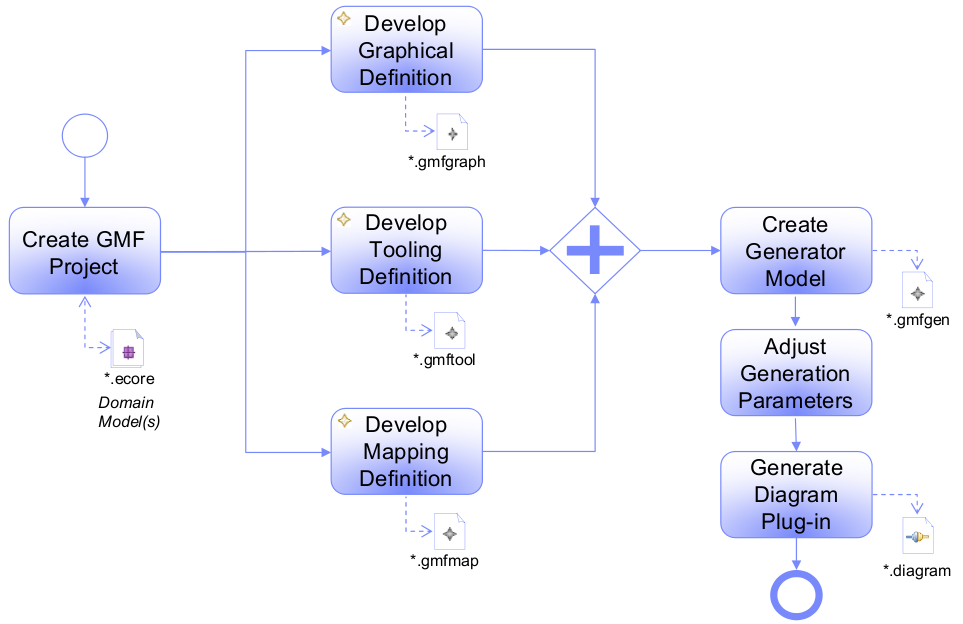
\includegraphics[scale=0.33]{gmf.png}
%   \end{center}
%   \caption{Exemplar usage of the Eclipse Graphical Modelling Framework.}
%   \label{fig:gmf}
% \end{figure}
% 
% Figure \ref{fig:gmf} illustrates the dependencies between the different types of model used to generate an editor with GMF. Should one model be changed, related models may also require migration to remain consistent.
% 
% GMF defines the metamodels for graphical, tooling and mapping definition models; and for generator models. The metamodels have changed considerably during the development of GMF. Some changes have caused a metmodel to become inconsistent with its models. Presently, migration is encoded in Java. Gronback \footnote{Private communication, 2008} has stated that the migration code is difficult to maintain.
% 
% \subsubsection{FPTC}

\subsubsection{Other data} % (fold)
\label{ssub:other_data}
As only a small number of candidate projects fulfil all of the requirements, I decided to collect additional data from alternative sources. Firstly, examples from related domains (e.g. object-oriented systems) may provide suitable date. Secondly, I have been collaborating with colleagues from two projects, both of which are using iterative and incremental model-driven development. Example data for both types of evolution will be available from these two projects.

\paragraph{Examples of evolution from object-oriented systems} % (fold)
\label{par:examples_of_evolution_from_object_oriented_systems}
Object-oriented programs use objects to construct systems. Every object is an instance of (at least) one class. A class is a description of characteristics, which are shared by each of the class's instances (objects).

This relationship between classes and objects is used in metamodelling. There, the term model element is used, instead of object, to refer to the individual parts of a model. Together, model elements are used to describe one perspective (model) of a system. Furthermore, metamodels comprises meta-classes, which describe the characteristics shared by each of the meta-class's instances (model elements).

Consequently, I believe that studying the evolution of object-oriented systems will yield results that are relevant to the model and metamodel co-evolution occurring in MDE. To support this argument, I have performed a preliminary study of frequently observed changes made to object-oriented systems.

\subparagraph{Preliminary study of object-oriented refactorings} % (fold)
\label{subp:preliminary_study_of_object_oriented_refactorings}
\emph{Refactoring} is the process of improving the structure of existing code while maintaining its external behaviour. When used as a noun, a refactoring is one such improvement. \cite{fowler99refactoring} provides a catalogue of \emph{refactorings} for object-oriented systems. For each refactoring, Fowler describes when it should be applied and instructions for applying it. 

Fowler's refactorings provide examples of evolutionary changes to object-oriented systems. I found that some of Fowler's refactorings can equally be applied to EMF metamodels, but many cannot. Broadly, those refactorings that do not apply to EMF metamodels belong to one of three categories:

\begin{enumerate}
	\item \textbf{Operational refactorings} focus on restructuring behaviour (method bodies). EMF does not support the specification of behaviour in models.
	\item \textbf{Navigational refactorings} convert, for example, between bi-directional and uni-directional associations. These changes are non-breaking in EMF, which automatically provides values for the inverse of a reference when required.
	\item \textbf{Domain-specific refactorings} manage issues specific to object-oriented programming, such as casting, defensive return values, and assertions. These issues are not relevant to modelling.
\end{enumerate}

Those refactorings that can be applied to metamodels provide examples of metamodel evolution. When applied, some of these refactorings can cause inconsistency between a metamodel and its models. I used Fowler's description of the refactoring to deduce a migration strategy for updating (co-evolving) inconsistent models. An example of deducing a migration strategy is now presented.

Figure \ref{fig:refactoring} illustrates a refactoring that changes a reference object to a value. Value objects are immutable, and cannot be shared (i.e. any two objects cannot refer to the same value object). Reference objects are mutable, and can be shared. Figure \ref{fig:refactoring} indicates that applying the refactoring restricts the multiplicity of the association (on the Order end) to 1 (implied by the composition); prior to the refactoring the multiplicity is many.

\begin{figure}[htbp]
  \begin{center}
    \leavevmode
    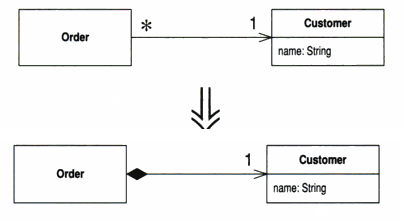
\includegraphics[scale=0.5]{refactoring.png}
  \end{center}
  \caption{Refactoring a reference to a value. Taken from \cite{fowler99refactoring}[pg183]}
  \label{fig:refactoring}
\end{figure}

Before applying the refactoring, every customer is associated with many orders. After the refactoring, each customer should be associated with only one order. Fowler indicates that every customer that is associated with more than one order should be replicated by the order. Therefore, the migration strategy in Listing \ref{lst:refactoring} is deduced.

\begin{lstlisting}[caption=Migration strategy for the above refactoring in pseudo code., label=lst:refactoring]
for every customer, c
	for every order, o, associated with c
		create a new customer, d
		copy the values of c's attributes into d
	next o
	
	delete c
next c
\end{lstlisting}

Migration strategies were deduced for each of the refactorings that were (1) applicable to metamodels, and (2) caused inconsistencies between a metamodel and its models. Some of the refactorings have been observed in the GMF and FPTC projects (both suitable candidates for the model and metamodel co-evolution study); although a thorough categorisation of the changes occurring in the projects has not been produced.

Object-oriented refactorings are used to improve the maintainability of existing systems. Consequently, they represent only one of the reasons for evolutionary change defined by \cite{sjoberg93quantifying}. Other types of changes to object-oriented systems are equally relevant to my research. Consequently, I have obtained further examples of changes made to object-oriented systems from Tim Hoverd, an experienced object-oriented developer. Hoverd's examples include changes made to adapt to new requirements and technologies.

% subparagraph preliminary_study_of_object_oriented_refactorings (end)
% paragraph examples_of_evolution_from_object_oriented_systems (end)


\paragraph{Collaborations} % (fold)
\label{par:collaborations}
With Adam, Heather.


% paragraph collaborations (end)

% TODO: Round up by describing why I have elected to focus on model and metamodel co-evolution.

% subsubsection other_data (end)



